% Middleware 2017 -- Sample Latex submission style

%\documentclass[sigplan, anonymous]{acmart}
\documentclass[sigplan]{acmart}

\usepackage{booktabs} % For formal tables

% Copyright
%\setcopyright{none}
%\setcopyright{acmcopyright}
%\setcopyright{acmlicensed}
% \setcopyright{rightsretained}
%\setcopyright{usgov}
%\setcopyright{usgovmixed}
%\setcopyright{cagov}
%\setcopyright{cagovmixed}

% DOI
% \acmDOI{10.475/123_4}

% ISBN
% \acmISBN{123-4567-24-567/08/06}

%Conference
\acmConference[Middleware'18]{ACM/IFIP/USENIX Middleware}{Dec 2018}{Rennes, France} 
\acmYear{2018}
\copyrightyear{2018}

% \acmPrice{15.00}

% \acmBadgeL[http://ctuning.org/ae/ppopp2016.html]{ae-logo}
% \acmBadgeR[http://ctuning.org/ae/ppopp2016.html]{ae-logo}

\begin{document}
\title{Metrological Surveillance of Fuel Dispensers using Blockchains}

\author{Wilson S. Melo Jr, \\Luiz F.R.C. Carmo}
%\orcid{1234-5678-9012}
\affiliation{%
  \institution{Federal University of Rio de Janeiro\\}
  %\streetaddress{P.O. Box 1212}
  \city{Rio de Janeiro} 
  \state{RJ}
  \country{Brazil}
  %\postcode{43017-6221}
}
\email{{wilson.junior,rust}@ppgi.ufrj.br}

\author{Alysson Bessani}
\affiliation{%
  \institution{LaSIGE, Faculdade de Ci\^encias\\}
  %\streetaddress{P.O. Box 1212}
  \city{Universidade de Lisboa} 
  \country{Portugal} 
  %\postcode{43017-6221}
}
\email{bessani@fc.ul.pt}

\author{Luiz Tarelho, \\Bruno Rodrigues Filho}
\affiliation{%
  \institution{Inmetro}
  %\streetaddress{1 Th{\o}rv{\"a}ld Circle}
  \city{Duque de Caxias} 
  \state{RJ}
  \country{Brazil}}
\email{{lvtarelho,bafilho}@inmetro.gov.br}

% The default list of authors is too long for headers}
\renewcommand{\shortauthors}{W. Melo Jr et al.}

\begin{abstract}
The abstract goes here. 
\end{abstract}

%
% The code below should be generated by the tool at
% http://dl.acm.org/ccs.cfm
% Please copy and paste the code instead of the example below. 
%
% \begin{CCSXML}
% <ccs2012>
%  <concept>
%   <concept_id>10010520.10010553.10010562</concept_id>
%   <concept_desc>Computer systems organization~Embedded systems</concept_desc>
%   <concept_significance>500</concept_significance>
%  </concept>
%  <concept>
%   <concept_id>10010520.10010575.10010755</concept_id>
%   <concept_desc>Computer systems organization~Redundancy</concept_desc>
%   <concept_significance>300</concept_significance>
%  </concept>
%  <concept>
%   <concept_id>10010520.10010553.10010554</concept_id>
%   <concept_desc>Computer systems organization~Robotics</concept_desc>
%   <concept_significance>100</concept_significance>
%  </concept>
%  <concept>
%   <concept_id>10003033.10003083.10003095</concept_id>
%   <concept_desc>Networks~Network reliability</concept_desc>
%   <concept_significance>100</concept_significance>
%  </concept>
% </ccs2012>  
% \end{CCSXML}

% \ccsdesc[500]{Computer systems organization~Embedded systems}
% \ccsdesc[300]{Computer systems organization~Redundancy}
% \ccsdesc{Computer systems organization~Robotics}
% \ccsdesc[100]{Networks~Network reliability}

% We no longer use \terms command
%\terms{Theory}

% \keywords{ACM proceedings, \LaTeX, text tagging}

\maketitle

\section{Introduction}

Fuel dispensers (or fuel pumps) are measuring instruments which play a crucial role in the trading of fuel as a consumable good.
In practically any place in the world, fuel stations and consumers trade fuel based on measurements given by fuel dispensers.
The transaction relies on the assumption that the fuel dispensers is a precise, accurate and reliable measuring instrument.
In fact, directives promoted by regulatory agencies and metrological supervision activities introduced by legal metrology are often employed for assuring such assumption.
However, in practice, evidence points that frauds against fuel dispensers are a growing and widespread practice, especially in developing countries.
One of the most common fraud is known as "low pump," and it occurs when the fuel dispenser delivers a fuel amount lower than the informed to the consumer.
Such practice affects an expressive percentual of trade transactions, resulting in significative economic losses for all the society.

The main problem associated with such frauds is the difficulty in proceeding with metrological supervision activities.
Although legal metrology usually designates notified bodies for inspecting fuel dispensers, these activities are not sufficiently efficient.
The high number of instruments spread over extensive geographic areas with high capillarity constitutes a challenge concerning logistic and inspection costs.
Also, many frauds employ sophisticated mechanisms which explore electronics and software features of the fuel dispenser.
These mechanisms can be activated and deactivated automatically, becoming the fraudulent behavior stealthy and hard for detecting.
Although there are several entities interested in solutions against such cheating (e.g., honest fuel station owners, fuel manufacturers, regulation agencies, and civil representatives), these frauds are very profitable.
That increases the chance of collusion among the dishonest fuel vendor and entities which could expose his fraudulent acts.

In this work, we propose a distributed and decentralized solution to deal with the described problem.
Our idea consists of using vehicles as sensors that perform an additional measuring of fuel in each refueling event and make this information available in a distributed data storage.
Although vehicles' sensors can be imprecise and inaccurate, the information collected by a large number of vehicles can be handy to indicate fraudulent behavior in fuel dispensers.
We demonstrate the statistical conditions that must be satisfied for reaching such results.
Besides, we propose the use of permissioned blockchains for storing information in a distributed way.
Once we have different stakeholders interested in preventing frauds in fuel dispensers, they efforts maintain a blockchain for metrological surveillance constitutes a robust solution against collusion agreements.

The main contributions in this paper are the following:
\begin{itemize}
 \item We present a statistical approach for performing metrological surveillance using measuring instruments whose uncertainty is unknown. That is an exciting result with several applications in legal metrology field. We validate our method by simulating refuel events based on real data collected in metrological supervision activities and inspections.
 \item We propose an abstract model and instantiate it in two implementation models: the regulated and the free surveillance schemes. We give particular attention to the free model, where vehicles can contribute to metrological surveillance actively and spontaneously. We also discuss the available technologies for obtaining fuel measurements from a vehicle's tank in refueling events.
 \item We describe and implement a blockchain network using HyperLedger Fabric for storing the measurements gathered from vehicles and fuel dispensers. We present a basic configuration involving different stakeholders and estimate the number of peers required to meet the demand in São Paulo state, in Brazil.
 \item We proceed with a comprehensive security analysis of the proposed solution. We show its main advantages and drawbacks, pointing out security techniques for preventing attacks increasing protection.
\end{itemize}

% \subsection{Topics}
% 
% \begin{itemize}
% \item Measurement frauds in fuel dispensers are very common.
% 
% \item They are more frequent in developing countries.
% 
% \item The costs associated to the prejudice of the society is estimated in \cite{RodriguesFilho2016}.
% 
% \item Although that is a serious problem, research works proposing security approaches and alternatives are scarce.
% 
% \item The majority of ideas are associated with patents and proprietary alternatives which the use is not spread out.
% 
% \item When we consider metrological authorities, ideas concerning product improvement or the use of information technology can make the difference.
% 
% \end{itemize}


% \subsection{Text Introduction}
% 
% Frauds against fuel dispensers or fuel pumps are widespread in developing countries.
% A tampered fuel pump usually delivers less fuel than the measured value informed to the client \cite{Luchsinger2008,Leitao2014,Leitao2014a,Beteto2016,RodriguesFilho2016}.
% We propose a metrological surveillance strategy based on additional measurements obtained from the vehicles' embedded computer (VEC).
% Although VEC measurements do not have metrological precision, we can use the unprecise measurements done by several vehicles to infer something about the fuel pump reliability.
% So we need a system that collects fuel measurements from vehicle in the refilling moment. Such information is kept together the metrological measurement obtained from the fuel pump.
% Such information is stored in a blockchain.
% Thus we assure its immutability, at the same time that we create a public environment for entities that want to implement data fraud analyses.
% 
% 
% The implementation of such systems needs to address some challenges:
% \begin{enumerate}
%  \item How can we be sure that VEC measurements come from the respective refilled vehicle?
%  \item How can this information be stored securely?
%  \item How can analysis inferences be implemented to detect a tampered fuel pump?
% \end{enumerate}
% 
% The problem can be described as follows. 
% We have a measuring instrument M whose the measurement uncertainty is a known value $I_M$.
% This instrument is under metrological control, which implies regulation and metrological supervision. 
% However, an attacker can tamper the instrument or even this measurements, compromising their accuracy and reliability.
% 
% Now, we assume we have a second measurement instrument N whose the measurement uncertainty $I_N$ is unknown.
% By comparing the measurements of each instrument, we cannot claim anything about the tampering of the first one. 
% However, it this same comparison is made using several instruments for different measurements...


% \subsection{Mind map for helping}
% We have a mind map in \emph{\href{https://mm.tt/973673423?t=Qtl0EQxNp2}{https://mm.tt/973673423?t=Qtl0EQxNp2}}. Everybody are invited to change and improve it to help the work.
% 
% \subsection{Create new sessions as necessary}
% Any new session (even a temporary one) can be created in this template. References shall be added in the file paper.bib, using bibtex format e referenced in the text as follows: \cite{Peters2015}.
% 
% One can make several citations together \cite{Zhang2016,Beteto2013,Beteto2016,RodriguesFilho2016,Luchsinger2008}.


\section{Preliminaries}

\subsection{Legal Metrology}

Legal metrology is responsible for the control of instruments that impact both the economy and society, according to each country's necessity. Due to regulation, countries established all the necessary levels of control regarding measuring instruments, especially in measurements where one or both parts have no means to check the accuracy of the measurement. Consequently, legal metrology acts as a third party assessor in order to make a measure reliable. Fuel dispensers are usually under the control of legal metrology since they have an important impact on every country´s economy. The levels of control in legal metrology can be described as (referencia VIML):

\begin{enumerate}

 \item Legal control of measuring instruments - Comprising the stages represented by type approval and both initial and subsequent verification of devices used on the market;
 \item Metrological supervision - Activities aiming to check the accordance of devices to metrology laws and regulations;
 \item The operations comprising examination and demonstration of conformity to a court for legal penalties, previously known as metrological expertise.

\end{enumerate}

Fuel dispensers are subject to subsequent verifications i.e, there are periodically tested and compared to volume standards applying procedures based on the international recommendations issued by the International Organization of Legal Metrology, OIML. 
They are also subjective of metrological supervision, where the equipment is supervised randomly on the market, checking the accordance to the legal requirements. The devices that do not fulfill the requirements are rejected and shall be removed from use.
Although all the legal metrology levels of control, the instruments are always subjective to metrological frauds, where the seller intentionally influence the performance of the instrument impacting in its accuracy due to a component of uncertainty against the buyer. In the fuel market, a simulation showed that for a 10 percent volume fraud and  1 percent fraudulent devices on the market, the economic losses are represented by approximately USD 300 million \citep{RodriguesFilho2016}. Another important aspect of frauds also relies on the unfair competition to the business that does not apply fraudulent procedures.

In Brazil, information technologies and management systems have been applied to legal metrology successfully, increasing the efficiency of the processes regarding all the levels of control \cite{RodriguesFilho2015a}, consequently optimizing the allocation of the resources in the legal control, bringing conformity and measurement assurance to the economy and fair trade to the society.

On the other hand, the usage of new technologies also raise still unknown issues, especially in legal metrology, which demands a certain level of security, preventing the fraudulent use of personal information. Traditional security systems has been showing to be failure when working in a connected and interactive networking, as in a smart city context \cite{Biswas2016}, and the blockchain technology has  been applied to surpass the security aspect.

\subsection{Technologies for Fuel Measurement}
\subsubsection{How fuel dispensers work}
An electronic fuel dispenser pumps the fuel from an underground tank passing into a measurement transducer, responsible for the measurement, throughout the nozzle, under the control of a solenoid valve, to the car tank. The measurement transducer is typically represented by a mechanical axis integrated to a pulser, where the movement of the axis is converted to electronic pulses, consequently the number of pulses is proportional to the measured volume. Figure \ref{f:transducer} shows an illustration of measurement transducer, as well as a typical fuel dispenser measurement transducer.

\begin{figure}[!t]
\centering
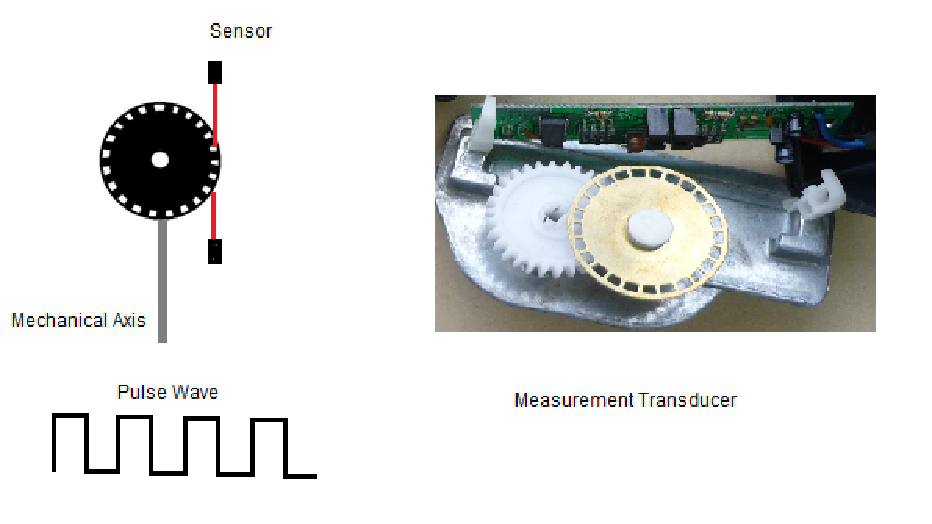
\includegraphics[width=.45\textwidth]{transducer}
\caption{Principle of a measurement transducer and a real device}
\label{f:transducer}
\end{figure}


According to the OIML International Recommendation (inserir referencia), the accuracy test comprises in testing the instrument in different flow rates using a standard capacity measure. For example, in Brazil, the test follows the recommendation where a 20 liters standard is used, and the maximum permissible error is 0.5 percent, for both maximum and minimum flow rate.


\subsubsection{Measuring fuel in vehicles}
Fuel amount estimation is an important requirement in different applications related to vehicles \cite{Skog2014,Obikoya2014,Andria2016,Kumar2017,Ahmed2017,Patil2017}.
We find such examples in telemetry, driver evaluation, fleet monitoring, and fuel thief prevention, among others.
In the majority of countries, it is mandatory that vehicles exhibit the fuel measurement to the driver.
The main reason is for preventing drivers from running out fuel.
Vehicles do that using different resources, since simple analogic fuel gauges until modern digital displays embedded in the vehicle's panel.
Some vehicle models also use fuel measurements to improve the engine performance \cite{Skog2014}.
However, most of the times, such embedded measuring instrument is not designed to be precise either accurate.
Thus these properties depend on the technologies used for measuring the fuel.

Level sensors are the most common technology behind vehicles' fuel measuring instruments \cite{Obikoya2014}.
There are also more sophisticated instruments that use ultrasound sensors or other non-intrusive technologies \cite{Ahmed2017,Patil2017}.
In industry, the decision about which technology to use is usually price-oriented.
Even so, recent works proposing low-cost vehicles' fuel meters report measuring errors no higher than 5\% \cite{Obikoya2014,Ahmed2017,Kumar2017,Patil2017}.

An important question is how one can collect the vehicle's fuel measurements.
OBD (Onboard Diagnostics) Protocol is an alternative for obtaining information from vehicle's embedded sensors \cite{Andria2016}.
OBD interfaces have been a mandatory requirement in vehicles produced in the USA and Europe for the last 15 years.
Nowadays one finds low-cost OBD monitoring devices are easily bought on the Internet. 
They can automatize information gathering from the vehicle by reading any available diagnosis information, including fuel measurements.
Smart sensors with communication features are also a suitable solution.
That enables the sensor to send fuel measurements directly to a monitoring application.
An example of such approach is given in \cite{Ahmed2017}.


\subsection{Physical Context-based Authentication}
Physical context-based authentication is a security strategy that uses physical context information shared among different entities to reinforce authentication process \cite{MeloJr.2018}.
Such mechanism can be used in two-factor authentication, being helpful to protect against external attacks (i.e., attackers which are not able to describe the specific physical context).
The basic idea is that entities describing a same physical event can use such information to generate a unique identifier.
In turn, this identifier can attest co-location and simultaneity among the entities.
It also can be used to generate shared secret keys for establishing a secure communication channel among authenticated entities.

\subsection{Methods for Data Analysis}
Principal Component Analysis (PCA) is the fundamental method and most commonly applied statistical procedure that uses an orthogonal transformation to convert a set of observations of possibly correlated variables into a set of values of linearly uncorrelated variables called "principal components" \cite{Peters2015}. The first principal component (PC) is defined by the spectral profile (loading) in the data which describes most of the variation and the second PC is the profile describing the second most of the variation orthogonal to the first and so on. The PC's are composed of so called scores and loadings. Scores and loadings have information about samples and variables, respectively, since they are analyzed together. Variation in the data which is not explained by the model is described in the residuals. The purpose of PCA is data reduction, facilitating an exploratory analysis.
Hierarchical cluster analysis (HCA) is an unsupervised technique for solving classification problems. HCA is a method of cluster analysis which seeks to build a hierarchy of clusters, commonly used in data mining and statistics. Its aim is to sort cases into clusters such that the degree of association is strong between members of the same cluster and weak between members of different clusters. In general, there are many choices of cluster analysis methodology. One of the the clustering method defines the cluster distance between two clusters to be the maximum distance between their individual components. At every stage of the clustering process, the two nearest clusters are merged into a new cluster. The process is repeated until the whole data set is agglomerated into one single cluster.
The support vector machines (SVM) is a supervised technique for solving classification problems based on the statistical learning theory and is applied to machine learning. SVMs are supervised learning models with associated learning algorithms that analyze data used for classification and regression analysis. When used for classification the method simultaneously minimizes the empirical error of classification and maximize the separation margin between classes using an optimal separation hyperplane, leading to an unique solution. One of the major features of SVC models is that they can operate in a kernel induced feature space allowing non-linear modeling and good generalization performance is obtained even with relatively small datasets. These characteristics can provide a better performance of SVC in relation to algorithms like as PCA and HCA.

\subsection{Blockchains}
Blockchain is an emerging technology which has called attention of stakeholders in different industry segments. 
Initially associated to crypto-currency markets due to Bitcoin popularity \cite{Zheng2017}, blockchain-based architectures have been proposed for a wide set of application areas including sensors networks, internet of things, smart cities, among others \cite{Zheng2017,Androulaki2018}.
%become one of the most promising technologies for the next generation of Internet interaction systems, such as smart contracts, public services, Internet of Things (IoT), reputation systems and security services

Conceptually, a blockchain can be regarded as a distributed append-only data structure (designated as \emph{ledger}) which is replicated and shared among a set of network peers \cite{Christidis2016}. 
This structure consists of a sequence of blocks where block $n$ is cryptographically linked to the block $n-1$ using a hash function. 
Consequently, block $n$ can not be changed without also modifying all subsequent blocks $n + i, ..., n + k$ \cite{Sousa2017}. 
%Being a decentralized model, blockchains availability does not depend on third parties, which can greatly save costs \cite{Zheng2017}.
By avoiding central points of control, blockchains availability does not depend on third parties, which can greatly save costs \cite{Zheng2017}.
In turn, integrity and availability are ensured by consensus among the peers, preventing the whole chain from being modified and requiring an agreement about any block to be appended to the ledger \cite{Sousa2017,Vukolic2016}. 
Blockchain platforms can be classified as \emph{permissionless}, when anybody can join to the network and participate in the network consensus, or \emph{permissioned}, when consensus is achieved by a set of known and identifiable peers \cite{Vukolic2016,Androulaki2018}. 
Usually, permissioned blockchains consensus protocols expend less computational resources and can reach better transaction latency and throughput \cite{Sousa2017}.
%REMOVIDO: One can say that blockchain enables trustless networks while using public key cryptographic for providing confidentiality and authenticity. 

A blockchain can store virtually any digital asset, from data to self-executing scripts, usually defined as \emph{smart contracts}. 
%Ethereum \cite{Christidis2016} is probably the most well-known blockchain implementation supporting that. 
That makes blockchain not only a data storage architecture but also a complete distributed platform for proper and distributed automated workflow \cite{Christidis2016}. 
%Once smart contracts are executed at every network peer in an independent and automatic manner, software integrity is achieved from blockchains integrity as a whole. 
%Such property has a remarkably impact over applications that requires software identification and integrity checking.

% Note that the IEEE does not put floats in the very first column
% - or typically anywhere on the first page for that matter. Also,
% in-text middle ("here") positioning is typically not used, but it
% is allowed and encouraged for Computer Society conferences (but
% not Computer Society journals). Most IEEE journals/conferences use
% top floats exclusively. 
% Note that, LaTeX2e, unlike IEEE journals/conferences, places
% footnotes above bottom floats. This can be corrected via the
% \fnbelowfloat command of the stfloats package.

% \section{Attack model}
% In a typical scenario involving vehicles and fuel dispensers, we assume that an attacker aims to get undue economic advantages by tampering the fuel measurements.
% Initially, one can consider any one of the parts involved in the commercial transaction as suspicious.
% However, in a simplified manner, we identify malicious drivers and fuel vendors as potential attackers.
% Malicious fuel vendors take advantage from cases when the fuel measurement is higher than the correct value.
% In opposite, a fuel measurement lower than the correct amount benefits malicious drivers. 
% 
% A malicious fuel vendor is expected to be more resourceful attacker. That happens because he is the formal owner of the devices used in the commercial transaction (e.g., fuel dispenser, payment systems).
% The fuel vendor can control and modify the devices features, compromising the measurements accuracy.
% 
% Malicious drivers also can tamper with measurements.
% However, they are limited when compared to fuel vendors.
% Although the driver has total control over the vehicle measuring system, it is the fuel dispenser which rules the commercial transaction.
% Any tampered measurement coming from the vehicle does not result in economic advantages.
% It is possible to consider individual cases where the driver hacks the fuel dispenser or the payment system.
% Even so, these are exceptional cases once these devices usually do not implement use cases that can be explored in such manner.
% 
% Alternatively, drivers can cheat with the vehicle measurement, aiming to create false suspicions about the fuel dispenser accuracy.
% Such attack succeeds only with collusion among a significative number of vehicles.
% Collusion attacks are typically expensive.
% Also, they do not result in economic advantages in this particular case.
% A more reasonable approach is forging false refueling events.
% The malicious driver generates a measurement by simulating a refuel. 
% After he notifies the surveillance, claiming that the fuel station did not report the event.
% We discuss that specific attack condition in a further section.
% 
% Due to the discussed aspects, we consider the attacker as malicious fuel vendors with the following capabilities:
% \begin{itemize}
%  \item The attacker can compromise the fuel dispenser measurement mechanism.
%  \item The attacker can modify electrical components in the fuel dispenser, consequently changing its measurement features.
%  \item The attacker can inject malicious software into the fuel dispenser, also compromising measurement information.
%  \item The attacker can tamper measurements when they are collected from the fuel dispenser.
%  \item The attacker can tamper measurements informed by the vehicle.
% \end{itemize}

\section{The Abstract Model}
\subsection{A basic metrological supervision framework}
Be $\mathcal{V}=\{v_1, ..., v_n\}$ and $\mathcal{C}=\{c_1, ..., c_m\}$ the sets which represent vendors and consumers, respectively.
Vendors and consumers perform trade transactions $\mathcal{T}$ related to measured goods.
Each vendor $v_n$ can trade with different consumers, as so each consumer $c_m$ can trade with several vendors.
%(Figure \ref{f:tradetrans}).

% \begin{figure}[!t]
% \centering
% 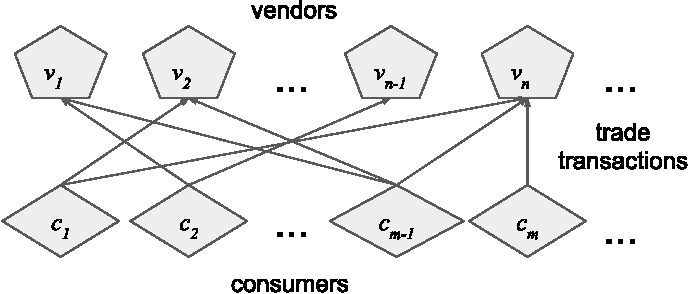
\includegraphics[width=.45\textwidth]{tradetrans}
% \caption{Trade transactions among vendors and consumers}
% \label{f:tradetrans}
% \end{figure}

Any trade transaction of measured goods can involve conflict of interests.
So we assume that, for each transaction $\mathcal{T}$, the respective vendor $v_n$ has a measuring instrument $\mathcal{M}_k$ which regulates the transaction by informing the correct measurement.
The measuring instrument $\mathcal{M}_k$ belongs to $v_n$ because he is the most interested in concluding the transaction and make profits from that.

In practice, $\mathcal{M}_k$ works as a third party, which provides reliability to the transaction $\mathcal{T}$. 
However, different factors can compromise $\mathcal{M}_k$'s precision and accuracy (e.g., unintentional fails, misbehavior, or even fraud attacks).
That is why legal metrology introduces the idea of \emph{metrological supervision}.
A basic supervision framework includes the role of a notified body $\mathcal{N}$ (Figure \ref{f:basicframe1}).
It is responsible for verifying each measuring instrument $\mathcal{M}_k$ following specific directives (e.g., periodic inspection).
One can say that $\mathcal{N}$ attests the correct behavior of $\mathcal{M}_k$.
He also is responsible for halting measuring instruments which do not satisfies precision and accuracy criteria, applying eventual penalties when it finds evidence of mismanagement or malicious behavior.

\begin{figure}[!t]
\centering
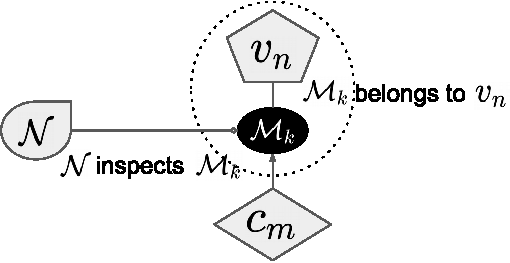
\includegraphics[width=.4\textwidth]{basicframe1}
\caption{A basic metrological supervision framework}
\label{f:basicframe1}
\end{figure}

\subsection{The problem}
The described model gives an overview about how legal metrology implements basic supervision frameworks in different places.
However, this framework presents several drawbacks in practice.

First, it requires \textit{in loco} instrument inspection, which forces $\mathcal{N}$ to travel to $\mathcal{M}_k$'s deployment site.
This scenario becomes even more expensive when instruments are in remote places, and their distribution presents a high capillarity.

Also, commercial transactions related to very profitable frauds can impose more challenging scenarios.
If $v_n$ or $c_m$ is a malicious entity, she can try to corrupt $\mathcal{N}$, offering bribes and convincing him to overlook inspection.
Furthermore, a modern $\mathcal{M}_k$ can be subject to sophisticated fraud mechanisms that switch the fraud behavior on or off when necessary.
Such attacks are harder to spot in conventional inspection procedures.

Different measures are taken to overcome such attacks.
That can involve physical sealing or tamper proof elements for protecting $\mathcal{M}_k$, or even inspection procedures that reduce the possibilities of $\mathcal{N}$ to be corrupted.
However, they are many times ineffective when the undue advantages exceed substantially the costs associated with the attack implementation.
Thus we need a more suitable idea to deal with such drawbacks straightforwardly.

\subsection{The distributed and decentralized supervision framework (DDSF)}
We propose an extension of the basic supervision framework which deals with the problems discussed in the previous section.
Such strategy consists of a distributed and decentralized data storage service $\mathcal{D}_s$ which keeps the record of any performed trade transaction.
We named it as \emph{Distributed and Decentralized Supervision Framework} (DDSF).

We assume two conditions as necessary for enhancing such idea:
\begin{enumerate}
 \item \textbf{There is a set of stakeholders interested in supporting the reliability of any trade transaction.} 
  Such premise is very realistic. 
  Cheating trade transactions affect not only the directly involved parts (i.e., vendors and consumers).
  They also harm several other actors related to the business chain.
  That can include other vendors who have losses due to unfair competition, government agencies which need to worry about more restrictive supervision policies, notified bodies that have more efforts with inspection procedures, and the society in general once the trade relations are under suspicion.
 \item \textbf{Each consumer has a second measuring instrument $\mathcal{S}_l$ which gives a complementary estimative of measurement   	related to the traded good.}
  Such requirement can sound a little complex a the beginning.
  Measuring instruments with high precision and accuracy are expensive.
  That is one of the main reasons why, in consumer relations, $\mathcal{M}_k$ usually belongs to a vendor $v_n$.
  However, a consumer $c_m$ usually want to be sure that $\mathcal{M}_k$ is measuring correctly.
  If $c_m$ has resources for using a measuring instrument $\mathcal{S}_l$ to verify $\mathcal{M}_k$, he likely will do that.
\end{enumerate}

Once such conditions are fulfilled, we can conceive DDSF as follows.
Vendors and consumers send their measurements (given by $\mathcal{M}_k$ and $\mathcal{S}_l$ respectively) to the data storage service $\mathcal{D}_s$ (Figure \ref{f:basicframe2}).
independent stakeholders maintain $\mathcal{D}_s$ collaboratively as a distributed service.
That assures $\mathcal{D}_s$ availability and integrity.
At the same time, the data storage can be read on anytime for any stakeholder interested in implementing metrological supervision using statistical data analyses.
Supervision is not an exclusive role for notified bodies anymore.
Actually, supervision becomes a decentralized and more effective process.

\begin{figure}[!t]
\centering
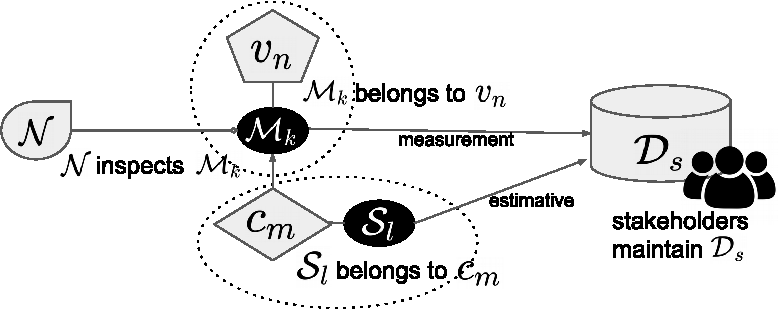
\includegraphics[width=.4\textwidth]{basicframe2}
\caption{The distributed metrological supervision framework (DMSF)}
\label{f:basicframe2}
\end{figure}

\subsection{How uncertainty affects DDSF}
An important question emerges from the DDSF idea.
It is related to how much precise and accurate $\mathcal{S}_l$ must be.
In other words, the metrological uncertainty associated with $\mathcal{S}_l$ measurements implies how useful this information could be for implementing statistical data analyses.

\textbf{TO-DO: Texto do Luiz Tarelho apresentando a fundamentacao teorica para fiscalizacao usando multiplas medicoes com incerteza desconhecida}.


\section{Instantiating the DDSF with Fuel Dispensers and Blockchain}
\subsection{The system overview}
In this section we instantiate the proposed DDSF to a real case which involves fuel measuring.
We glimpse a system for decentralized and distributed surveillance which uses vehicles as active sensors for providing information about fuel dispensers accuracy.
Vendors and consumers are respectively represented by fuel station owners and drivers.
In turn, $\mathcal{M}_k$ correspond to a fuel dispenser with expected high accuracy and precision, and $s_l$ is a vehicular measuring system whose accuracy and precision are totally unknown.
The data repository $\mathcal{D}_s$ is maintained for independent stakeholders, which can include other full station owners, government agencies, notified bodies, and entities representing consumer's interests.
$\mathcal{D}_s$ stores measurements records, which are basically the fuel measurements from fuel dispensers and vehicles, as so as any complementary information.
Authorized stakeholders can access such measurements and implement data analysis, contributing to surveillance in a comprehensive manner.

%We propose and evaluate such system starting from a conceptual model which describes the main idea.
%After describing such conceptual model, we can also discuss an attack model.
%The final solution is designed considering attacks and countermeasures.

Initially, we assume that each vehicle has a mechanism for estimating the fuel amount inside its fuel tank.
On each refueling, the difference between initial and final fuel quantities gives the refueling estimative, which correspond to the $s_l$'s measurement.
Although such estimative is expected to be inaccurate, a large number of estimative from different vehicles and refuel events can be handy to point out eventual fails or even frauds in fuel dispensers.

Different solution models can implement the described system.
We consider in this work two models which are conceptually different.
The first is based on rules which are imposed by a regulation authority, which obligates fuel station owners and drivers to send information to the system. We call it \emph{regulated model}.
The second model comes from the idea that correct fuel station owners and drivers have strong motivation to cooperate with the system.
So we assume a scenario where they voluntarily inform their respective measurements.
We call that as \emph{free model}.
In the next sections, we describe and compare both models.

\subsubsection{The regulated model}

%Figure~\ref{f:reg-free}~a shows an initial model that partially depicts some ideas already proposed in the literature \cite{Beteto2016}.
% \begin{figure}[!t]
% \centering
% 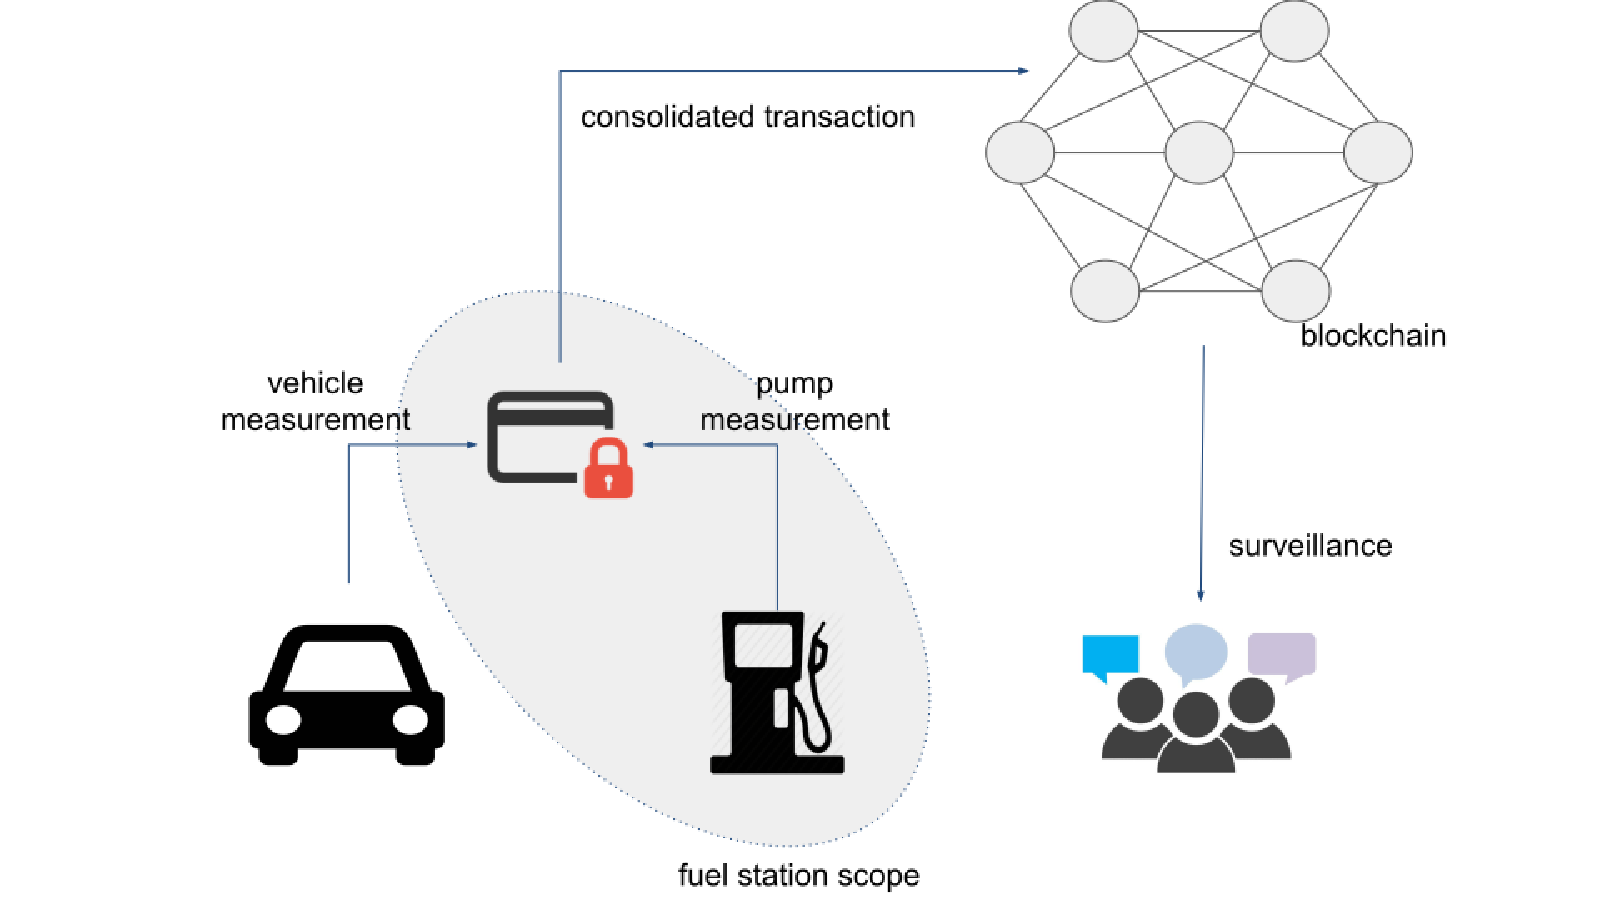
\includegraphics[width=.5\textwidth]{regulated}
% \caption{The Regulated Model}
% \label{f:regulated}
% \end{figure}

The regulated model comes from the assumption that both $\mathcal{M}_k$ and $s_l$ are obligated to inform the fuel measurement (and estimative) to the surveillance system.
Figure~\ref{f:reg-free}~a depicts the main associated ideas.
In the regulated model, the driver provides his vehicle's fuel measurement whenever a commercial transaction is committed.
After, the fuel vendor is responsible for sending the complete refuel measurement record to the blockchain network.
There are exceptional cases when the vehicle can not inform any measure, or when the driver refuses to provide such information.
However, for preventing malicious vendors from sending only the fuel dispenser measurement, or even do not send any information, the model introduces a trusted, tamper-proof, secure device (SD).
SD is responsible for collecting information from both traders.
After that, it commits the commercial transaction and stores the measurement record in the data repository.
One shall note that this idea is very similar to the solution proposed in \cite{Beteto2016}. The difference is that our model adds the vehicle's fuel measurements.  

The regulated model introduces advantages and drawbacks.
An advantage is that the SD can aggregate additional features for other regulatory bodies. 
For instance, the system can integrate tax payment surveillance once the SD manages prices and payments information \cite{Beteto2016}. 
On the other hand, solutions based on compulsory mechanisms tend to be more expensive.
It requires a complete infrastructure which includes the SD itself, a permanent communication link and fault-tolerant mechanisms for ensuring system availability and redundancy.
Also, SD belongs to the same scope that the fuel dispenser, which means that both are under control of the same entity.
If we assume that the fuel dispenser is under attack of a malicious entity, consequently the SD is subject to the same class of attacks.

\subsubsection{The free model}
\label{s:freemodel}
In contrast to the regulated model, we present the idea of a \emph{free model} (Figure~\ref{f:reg-free}~b).
Fundamentally, the difference is the manner how drivers and fuel vendors interact with the surveillance system.
In the free model, drivers and fuel vendors are invited to contribute voluntarily.
That concept takes advantage of common sense that correct entities have a strong motivation for exposing frauds.

\begin{figure*}[!t]
\centering
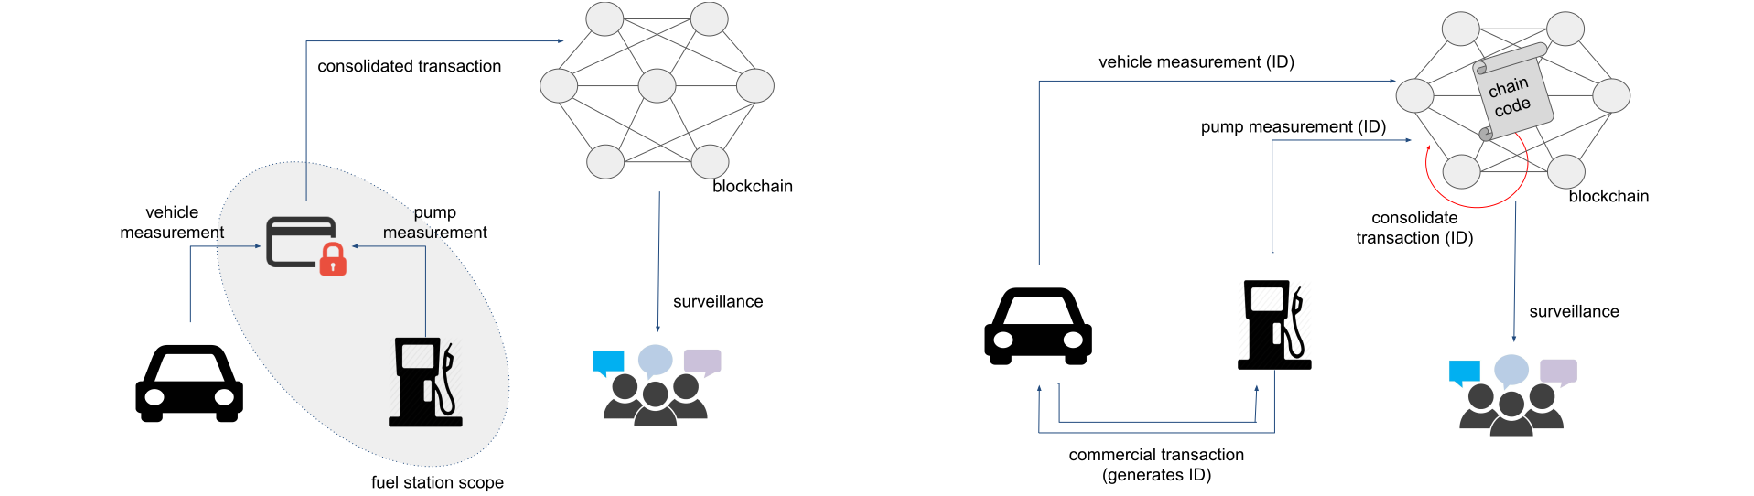
\includegraphics[width=.95\textwidth]{reg-free}
\caption{Comparing a) the regulated model and b) the free model}
\label{f:reg-free}
\end{figure*}

The free model works as follows.
Firstly, driver and vendor need to agree on a transaction ID to identify the refueling event. 
After that, they send their fuel measurement to the surveillance system in independent transactions linked by the same ID. 
%In turn, the blockchain network implements a smart contract and invokes it whenever two measurements with the same ID are received, or after a specific timeout.
The surveillance system consolidates both transactions, making the measurement record available to stakeholders.
Such approach is more straightforward than in the regulated model.
However, it results in three distinct possible scenarios.
The best one is when driver and vendor contribute to the system, sending their respective measurements.
The other scenarios occur when only one of the entities sends his measurement.
If only the vendor informs the fuel dispenser measurement, such information does not have a practical use because one does not have the vehicle measurement for comparing.
In turn, when only the driver informs the vehicle measurement, he also can tell the fuel dispenser measurement.
He knows this information once he asked the refueling and paid for it.
Although such measurement record could seem suspicious (i.e., the driver can cheat with the fuel dispenser measurement), it is yet useful for statistical analyses.

\subsection{Vehicle measurements and reliability}
The proposed surveillance system depends on the gathering of measurements from both fuel dispensers and vehicles.
One can do that in different manners, according to the employed technology.
In turn, the selected technology impacts the information reliability.
Even in cases when there are no frauds, information can be compromised due to the information gathering method.

Regarding measurements, fuel dispensers are expected to be very precise and accurate.
Some modern models also include features for increasing security (e.g., pulsers can provide the measurement's digital signature).
Besides, fuel dispensers also present a high automation level.
They commonly integrate with payment or data gathering systems for commercial automation.
Thus we can assume that the measurements provided for a non-malicious fuel vendor are highly reliable.

That does not happen with vehicles embedded measuring instruments.
In the majority of cases, accuracy and precision of such instruments are unknown.
The chosen gathering method also impacts on those properties.
We identify at least three different levels of reliability, according to the employed gathering methods.
We describe them as follows:
\begin{enumerate}
 \item User level. The user does the measurement gathering. 
  Essentially, the driver checks the measurement (e.g., a fuel level gauge or a display in the vehicle panel) and informs it to the surveillance system. 
  Such method has serious implications related to accuracy and reliability.
  For instance, a measurement from an analogic gauge is very imprecise and even hard to read.
  Even a non-malicious driver can inform a wrong measurement unintentionally.
  That is the less reliable level of a collected measurement.
  \item Middleware level. The vehicle has an interface that enables the measurement gathering.
  In this level, the user interaction is not necessary.
  A middleware gathers measurements from the vehicle's embedded computer using specific protocols and sends them to the surveillance system.
  Although reading errors become negligible,  the measurement reliability yet depends on the middleware features.
  One can adopt different security strategies for assuring measurements integrity and authenticity.
  However, such solutions aggregate complexity.
  We classify that as a quasi-reliable method.
  \item Fully integrate level: The vehicle has smart sensor into its vehicle fuel tank.
  The sensor delivers a fair, accurate measurement directly to the system surveillance.
  There is no need for interaction with the vehicle's embedded computer neither with the user.
  Furthermore, the sensor can use cryptographic mechanisms for assuring the measurement integrity and authenticity.
  %The sensor can even format the blockchain transaction, working as an oracle.
  This gathering method is the most reliable.
  However, it also implies a not simple solution.
  There are costs associated with the smart sensor acquisition,  deployment, and eventual maintaining.\end{enumerate}


\subsection{Metrological assurance}
\textbf{TO-DO: Texto do Luiz Tarelho descrevendo as condicoes teoricas que devem ser satisfeitas para que os dados de abastecimento do veiculo possam ser uteis na identificacao de eventuais fraudes.
}

\subsection{Cyber-physical security}
\textbf{TO-DO: Texto do Wilson argumentando como a seguranca ciber fisica do sistema e obtida.
Devem ser enfatizados os aspectos de seguranca intrinsecos ao blockchain e tambem os casos que justificam a autenticacao baseada em contexto fisico entre veiculo e bomba de combustivel.
}

\section{Security analysis}
\subsection{Identifying attackers and goals}
In a typical scenario involving vehicles and fuel dispensers, we assume that an attacker's primary objective is to get undue economic advantages.
He does that by tampering with fuel measurements.
Initially, one can consider suspicious any one of the parts involved in the commercial transaction.
However, in a simplified manner, we identify malicious drivers and fuel vendors as potential attackers.
Malicious fuel vendors take advantage from cases when the fuel measurement is higher than the correct value.
In opposite, a fuel measurement lower than the correct amount benefits malicious drivers.
Also, a scenario that contemplates a surveillance system introduces a second attack goal: the intention of compromise such system.
Primarily, a surveillance system evaluates the accuracy and correct behavior of fuel dispensers.
Thus a malicious fuel vendor tries to fool such system, creating the impression that his fuel dispensers are working correctly.
Malicious drivers can also target the surveillance system, aiming to create false suspicions about the fuel dispenser accuracy.

Regarding attack capabilities, a malicious fuel vendor is supposed to be more resourceful than a malicious driver. 
That happens because he is the formal owner of the devices used in the commercial transaction (e.g., fuel dispenser, payment systems).
The fuel vendor can control and modify these devices features, compromising the measurements accuracy.
Besides, fuel measurement frauds are very profitable for malicious vendors.
That motivates the conception of sophisticated attacks involving different components and devices. 

Malicious drivers also can tamper with measurements.
However, they are limited when compared to fuel vendors.
Although the driver has total control over the vehicle measuring system, it is the fuel dispenser which rules the commercial transaction.
Any tampered measurement coming from the vehicle does not result in economic advantages.
Although, one can consider exceptional cases where the driver can hack fuel dispensers or payment systems.

In turn, attacks targeting the surveillance system require still more specific resources.
We foresee two basic strategies: a) provide incorrect information in a manner that the surveillance system does not detect the measurement frauds and b) compromise the surveillance system itself, by tampering with the stored measurements.
Both strategies depend on collusion among fuel vendors, drivers, and even other stakeholders.
Collusion attacks are typically expensive.
Also, such attacks result in economic advantages only for fuel vendors.
That reduces the incentives for malicious drivers to take part in the collusion.
However, a possible attack approach is to generate false refueling events.
For instance, a malicious driver can forge several measurements,  creating fake refuel events.
After, he sends the information to the surveillance system, claiming that the fuel station did not report the event.

\subsection{Countermeasures}
We claim that the DDSF offers natural protection against several scenarios related to the described attacks.
One can observe different advantages and drawbacks when comparing the regulated and the free models.
We show that by evaluating the security features provided by each model in four main attack classes: measurement tampering, information denying, information forging and collusion.

\subsubsection{Measuring tampering}
Both regulated and free model try to detect frauds by counterposing measurements from the fuel vendor and the driver.
However, the regulated model depends on SD integrity and reliability.
If an attacker compromises SD, any collected measurement can be modified and tampered without any chance of detection.

One conceives the SD as a tamper-proofing device.
Consequently, any tentative of violating it is expected to be exposed.
However, we remember that legal metrology already enforces mechanisms for protecting fuel dispensers' integrity and ensuring their reliability.
Nevertheless, the high number of cases reporting metrological frauds in fuel dispensers shows that such assumption can fail.
The main problem is that the fuel dispenser is under control of a fuel vendor who can modify its behavior.
One must admit that the same can happen with SD.
Malicious fuel vendors can compromise SD integrity as so as they do with fuel dispensers.

On the other hand, the free model is robust against such attacks because it does not require any intermediate device for processing information before sending it to DDSF.
Although attackers can yet tamper with measurements, such practice may be exposed later by analyzing data in the blockchain using statistical heuristics (see section XX).

\subsubsection{Information Denying}
Information denying occurs when either the fuel vendor or the driver decides to omit information about a trading transaction.
The regulated model does not allow this class of attacks once the SD forces driver and fuel vendor to provide their measurements before committing the trading transaction.
There are some particular cases when the driver does not have any instrument for providing measurements.
In these cases, the driver shall agree with the fuel dispenser measurement and the trading transaction is considered correct.
Also, we have scenarios where a compromised SD omits the measurement informed by the driver.
However, we consider such cases as a variant of the first class of attacks.

In contrast, such attack can be widespread and even stealthy in the free model.
Malicious fuel vendors can omit information purposely for hiding a fraudulent trading transaction.
In turn, drivers do not have any advantage in omitting information.
Notwithstanding,  they eventually may not have the necessary resources to do that, or simply decide not to contribute to the system.
Such choices are intrinsic to the nature of the free model.

Although information denying is supposed to be quite common in the free model, there is a practical manner of dealing with it: DDSF can consider as suspicious any transaction informed only by the driver.
That is a practical approach since fuel vendors are expected to have plenty of resources to send their information to the system.
However, that also introduces a new class of attacks, which consists in the possibility of an attacker to forge false transactions.

\subsubsection{Information forging}
Information forging happens when the attacker creates information about a false trading transaction.
Primarily, this kind of attack aims to compromise DDSF credibility.
Information from transactions that in fact did not happen can affect the statistical analysis and hazard DDSF efficiency.

In the regulated model, such attacks can be launched only by malicious fuel vendors because they require a compromised SD.
Also, we can not identify any advantage for fuel vendors in such attacks.
If a fuel vendor simulates a trading transaction, he does not harm any consumer.
In opposite, he can have problems with other authorities that can investigate if the amount of trading fuel corresponds to the amount of paid taxes.

In the free model, both fuel vendor and driver can try such attacks.
How we argue before, fuel vendors do not have any advantage in doing that.
Though drivers can try such attack aiming to spoil DDSF or even for harming the reputation of a correct fuel vendor.
The question is that an attack launched by only one driver is not enough to affect statistical analyses.
Also, we can easily spot transactions forged by the same driver, once they have the same user identification.
That invalidates the possibilities for a regular driver to undertake such attacks.

Finally, we consider one last possibility in the free model.
A resourceful attacker can personify different drivers by creating fake profiles or even stealing legitimate drivers identification.
Despite its chances of success, this attack is remarkably costly.
Also, we understand that such problem is related to the security of the system which assigns drivers' credentials.
Countermeasures can include the analysis of drivers behavior and the existence of a legal process for accepting drivers who want to join DDSF.

\subsubsection{Collusion attacks}
Collusion attacks are usually frequent in the context of fuel trading transactions.
The main reason is the fraud profitability.
Malicious fuel vendors can offer bribes to notified bodies and other legal authorities.
Groups of malicious vendors can even form cartels that control fuel prices and disseminate measurement frauds in large scale.
That is an admittedly tricky problem, whose the solution is not trivial.

Collusion attacks can occur in both regulated and free model.
However, there is an important difference.
In the regulated model, collusion can be used to commit frauds before and after the SD sends the measurement to the blockchain.
Collusion before sending information incurs in the same attacks already described for the SD.
The essential difference is that notified bodies or any other authorities taking part in the collusion consent with such attacks.
In contrast, collusion attacks in the free model only make sense after driver and fuel vendor sending their respective measurements.
Consequently, any collusion attack takes place against the blockchain.
The good news is that, in this context, blockchains play a crucial role against collusion attacks.

Blockchains work as a genuinely distributed and decentralized data store system.
That significantly reduces the possibility of a specific entity to take control of the network peers majority.
In a permissioned blockchain, the consensus decision is reached by a quorum of peers that belongs to independent organizations which are interested in fighting against frauds.
That forces an attacker to have the control of at least half of the peers that integrate the quorum, and consequently to form collusion with a significant number of people and organizations.
The more organizations participate in the consensus quorum, the more expensive the attack becomes.
Furthermore, blockchains constitute an append-only data storage architecture.
Once any information is stored, it is virtually impossible to modify or remove it.
That makes blockchains a singular technology for storing information used to detect and prevent measurement frauds.
Also, the extensive use of cryptographic features assures information authenticity and integrity.

% False suspicions usually impact much more fuel vendors than drivers.
% They can harm the reputation of a correct fuel vendor, besides result in wasting inspection resources.
% 
% We can use the text about capabilities later.
% 
% Considering all the aspects above, we define that a malicious fuel vendor has following attack capabilities:
% - The vendor can compromise the fuel dispenser measuring mechanism. That includes changing components (e.g., mechanical, electronics and software).
% - The vendor can tamper with measurements after collecting them from the fuel dispenser.
% - The vendor can compromise any middleware or management system (e.g., payment system). That implies to tamper with measurements from both vehicle and fuel dispenser.
% - The vendor can provide tampered information to the surveillance system.
% - The vendor can collude with other stakeholders to compromise the surveillance system integrity.
% 
% In complement, we define that a malicious driver has the following attack capabilities:
% - The driver can compromise the vehicle's measuring mechanism.
% - The driver can tamper with measurements



\section{Case Study: Experiment based on field surveillance data}
In this section, we develop a case study using field surveillance data collected by the National Institute of Metrology, Quality, and Technology (Inmetro).
Inmetro is the notified body responsible for type approval, market and field surveillance activities in Brazil.
TODO: ACRESCENTAR DADOS DE FISCALIZAÇÃO DO INMETRO

\subsection{Data simulation}
We start our experiment by simulating random refilling events.
The measurement error follows a normal distribution given by the mean and the standard deviation which we found in field surveillance activities.

We simulate refilling events considering scenarios with different numbers of vehicles and fuel dispensers.
In each scenario, we assign a different measurement uncertainty to the vehicles.
We also assume different tampered fuel dispensers percentages.
Our method accuracy is sensitive to these values.
A high number of tampered fuel dispensers increases false positives and false negatives rates.
The same happens when the vehicle's fuel measuring instrument has a high uncertainty.

\subsection{Analysis Heuristic}
Our experiment implements a statistical analysis based on the Law of the Large Numbers.
It tries to estimate the vehicle's measuring instrument uncertainty.
Firstly, we assume all the fuel dispensers as accurate and precise instruments.
Doing that, we can collect a set of refilling events and calculate the vehicle's measuring instrument uncertainty.
The more events we compute, the more precise the uncertainty estimate is.
%For each new refilling event, we can also update the vehicle's measuring instrument uncertainty.

After we have the vehicle's MI uncertainty, we can use it to evaluate new refilling events.
That is our first level analysis.
For each vehicle, we use the mean and the standard deviation of the refilling events to identify outliers.
We then insert the fuel dispensers associated with these events in a suspicion list.
The second level analysis collects the suspicion list of each vehicle and computes the total of suspicion occurrences of each fuel dispenser.
Again, we use the mean and the standard deviation of the suspicion list, but now discarding outliers and considering the more frequent fuel dispensers as suspicious of fraud.

We implement the analysis heuristic using Go language.
The code runs as a smart contract in a blockchain-based DDSF.
We describe our blockchain architecture in the next section.

% \textbf{TO-DO: Texto do Luiz Tarelho descrevendo como os dados de simulacao de reabastecimento foram gerados.
% Deve englobar os seguintes topicos:
% \begin{itemize}
%  \item Dados de fiscalizacao usados na estimativa da distribuicao do erro de medicao.
%  \item Numero de amostras e estrutura dos dados simulado.
%  \item Ferramentas computacionais utilizadas na simulacao.
% \end{itemize}
% }

\subsection{The Blockchain Implementation}
We use HyperLedger Fabric in our experiment.
Fabric is an open source platform for implementing permissioned blockchains \cite{Androulaki2018}.
We develop a blockchain network where the organizations represent stakeholders which are co-operating with the DDSF solution.
Each organization provides a respective number of peers that constitutes the blockchain network.
Some organizations also take part in the orderer consortium (i.e., a group of peers that performs the blockchain consensus using BFT protocols).
We employed the BFT-SMART implementation described in \cite{Sousa2017}.

Figure X depicts our blockchain architecture. 
We consider two independent organizations (LaSIGE and Inmetro) providing each one a set of 4 ordinary peers and 2 consensus peers.
The DDSF follows the \emph{free model} idea described in the previous section.
The blockchain network accepts transactions from clients who are essentially vendors (i.e., fuel station owners) or consumers (i.e., drivers).
Every time a refilling event happens, the fuel dispenser generates an event ID.
This ID is unique and both clients use this ID to identify and send their measurements to the blockchain-based DDSF.
Thus the clients operate according to the steps described at the section \ref{s:freemodel}

We do not specify how fuel vendors send their transactions to the blockchain.
One shall consider that fuel dispenser are instruments which already can include resources for communicating and generate transactions.
On the other hands, the manner how consumers can contribute to DDSF is crucial.
That need to be done in a natural, practical way.
So we assume the existence of a smartphone app which can easily be used by consumers to generate transactions.
The app works in three different modes which correspond to the reliability levels described previously.
The consumer can choose one of them, in accordance with much he is interested in investing to help in fails and fraud detection.
These modes are:
\begin{itemize}
 \item Informative: the consumer texts the measurement informed by the fuel dispenser and also the measurement provided by his vehicle fuel gauge/panel. This mode does not imply any cost to the consumer.
 \item Measured by the vehicle system: the app connects to the vehicle using Bluetooth or OBD technologies and gets the fuel amount estimative provided by the vehicle's embedded computer. This mode can require an OBD adaptor (in case of the vehicle does not offer a Bluetooth interface) and perhaps some specialized training for configuring the app.
 \item Measured by smart sensors: the app connects to a smart sensor installed into the vehicle's fuel tank. The smart sensor provides highly accurate measurement and also signs such information, attesting to its authenticity. This mode requires more investment than the others.
 Smart sensors can be expensive, and its deployment usually requires a specialized service.
\end{itemize}

\subsection{Analysis results}
\textbf{TO-DO: Texto do Luiz Tarelho descrevendo como foi conduzida a analise dos dados simulados para tentar se identificar os instrumentos fraudados.
Deve englobar os seguintes topicos:
\begin{itemize}
 \item Metodo aplicado (ou metodos, caso mais de um).
 \item Matriz de confusao para diferentes volumes de dados.
 \item Analise dos resultados obtidos.
 \item Graficos sao bem vindos!
\end{itemize}
}

\section{Discussion of Results}
\textbf{TO-DO: Texto a ser elaborado em conjunto pelo grupo, enfatizando as vantagens e desvantagens de tal abordagem, reforcando as principais contribuicoes e definindo pontos que sao passiveis de melhoria.}

\section{Conclusion}
The conclusion goes here.

\bibliographystyle{ACM-Reference-Format}
\bibliography{paper} 

\end{document}
